%% iTrustInterviews.tex
%% V1.4
%% 2012/12/27
%% by Michael Shell
%% See:
%% http://www.michaelshell.org/
%% for current contact information.
%%
%% This is a skeleton file demonstrating the use of IEEEtran.cls
%% (requires IEEEtran.cls version 1.8 or later) with an IEEE conference paper.
%%
%% Support sites:
%% http://www.michaelshell.org/tex/ieeetran/
%% http://www.ctan.org/tex-archive/macros/latex/contrib/IEEEtran/
%% and
%% http://www.ieee.org/

%%*************************************************************************
%% Legal Notice:
%% This code is offered as-is without any warranty either expressed or
%% implied; without even the implied warranty of MERCHANTABILITY or
%% FITNESS FOR A PARTICULAR PURPOSE! 
%% User assumes all risk.
%% In no event shall IEEE or any contributor to this code be liable for
%% any damages or losses, including, but not limited to, incidental,
%% consequential, or any other damages, resulting from the use or misuse
%% of any information contained here.
%%
%% All comments are the opinions of their respective authors and are not
%% necessarily endorsed by the IEEE.
%%
%% This work is distributed under the LaTeX Project Public License (LPPL)
%% ( http://www.latex-project.org/ ) version 1.3, and may be freely used,
%% distributed and modified. A copy of the LPPL, version 1.3, is included
%% in the base LaTeX documentation of all distributions of LaTeX released
%% 2003/12/01 or later.
%% Retain all contribution notices and credits.
%% ** Modified files should be clearly indicated as such, including  **
%% ** renaming them and changing author support contact information. **
%%
%% File list of work: IEEEtran.cls, IEEEtran_HOWTO.pdf, bare_adv.tex,
%%                    bare_conf.tex, bare_jrnl.tex, bare_jrnl_compsoc.tex,
%%                    bare_jrnl_transmag.tex
%%*************************************************************************

% *** Authors should verify (and, if needed, correct) their LaTeX system  ***
% *** with the testflow diagnostic prior to trusting their LaTeX platform ***
% *** with production work. IEEE's font choices can trigger bugs that do  ***
% *** not appear when using other class files.                            ***
% The testflow support page is at:
% http://www.michaelshell.org/tex/testflow/



% Note that the a4paper option is mainly intended so that authors in
% countries using A4 can easily print to A4 and see how their papers will
% look in print - the typesetting of the document will not typically be
% affected with changes in paper size (but the bottom and side margins will).
% Use the testflow package mentioned above to verify correct handling of
% both paper sizes by the user's LaTeX system.
%
% Also note that the "draftcls" or "draftclsnofoot", not "draft", option
% should be used if it is desired that the figures are to be displayed in
% draft mode.
%
\documentclass[conference]{IEEEtran}
% Add the compsoc option for Computer Society conferences.
%
% If IEEEtran.cls has not been installed into the LaTeX system files,
% manually specify the path to it like:
% \documentclass[conference]{../sty/IEEEtran}





% Some very useful LaTeX packages include:
% (uncomment the ones you want to load)


% *** MISC UTILITY PACKAGES ***
%
%\usepackage{ifpdf}
% Heiko Oberdiek's ifpdf.sty is very useful if you need conditional
% compilation based on whether the output is pdf or dvi.
% usage:
% \ifpdf
%   % pdf code
% \else
%   % dvi code
% \fi
% The latest version of ifpdf.sty can be obtained from:
% http://www.ctan.org/tex-archive/macros/latex/contrib/oberdiek/
% Also, note that IEEEtran.cls V1.7 and later provides a builtin
% \ifCLASSINFOpdf conditional that works the same way.
% When switching from latex to pdflatex and vice-versa, the compiler may
% have to be run twice to clear warning/error messages.






% *** CITATION PACKAGES ***
%
\usepackage{cite}
% cite.sty was written by Donald Arseneau
% V1.6 and later of IEEEtran pre-defines the format of the cite.sty package
% \cite{} output to follow that of IEEE. Loading the cite package will
% result in citation numbers being automatically sorted and properly
% "compressed/ranged". e.g., [1], [9], [2], [7], [5], [6] without using
% cite.sty will become [1], [2], [5]--[7], [9] using cite.sty. cite.sty's
% \cite will automatically add leading space, if needed. Use cite.sty's
% noadjust option (cite.sty V3.8 and later) if you want to turn this off
% such as if a citation ever needs to be enclosed in parenthesis.
% cite.sty is already installed on most LaTeX systems. Be sure and use
% version 4.0 (2003-05-27) and later if using hyperref.sty. cite.sty does
% not currently provide for hyperlinked citations.
% The latest version can be obtained at:
% http://www.ctan.org/tex-archive/macros/latex/contrib/cite/
% The documentation is contained in the cite.sty file itself.





% *** GRAPHICS RELATED PACKAGES ***
%
\ifCLASSINFOpdf
   \usepackage[pdftex]{graphicx}
  % declare the path(s) where your graphic files are
   \graphicspath{{Images/}}
  % and their extensions so you won't have to specify these with
  % every instance of \includegraphics
   \DeclareGraphicsExtensions{.pdf,.jpeg,.png}
\else
  % or other class option (dvipsone, dvipdf, if not using dvips). graphicx
  % will default to the driver specified in the system graphics.cfg if no
  % driver is specified.
  % \usepackage[dvips]{graphicx}
  % declare the path(s) where your graphic files are
  % \graphicspath{{../eps/}}
  % and their extensions so you won't have to specify these with
  % every instance of \includegraphics
  % \DeclareGraphicsExtensions{.eps}
\fi
% graphicx was written by David Carlisle and Sebastian Rahtz. It is
% required if you want graphics, photos, etc. graphicx.sty is already
% installed on most LaTeX systems. The latest version and documentation
% can be obtained at: 
% http://www.ctan.org/tex-archive/macros/latex/required/graphics/
% Another good source of documentation is "Using Imported Graphics in
% LaTeX2e" by Keith Reckdahl which can be found at:
% http://www.ctan.org/tex-archive/info/epslatex/
%
% latex, and pdflatex in dvi mode, support graphics in encapsulated
% postscript (.eps) format. pdflatex in pdf mode supports graphics
% in .pdf, .jpeg, .png and .mps (metapost) formats. Users should ensure
% that all non-photo figures use a vector format (.eps, .pdf, .mps) and
% not a bitmapped formats (.jpeg, .png). IEEE frowns on bitmapped formats
% which can result in "jaggedy"/blurry rendering of lines and letters as
% well as large increases in file sizes.
%
% You can find documentation about the pdfTeX application at:
% http://www.tug.org/applications/pdftex


% correct bad hyphenation here
\hyphenation{op-tical net-works semi-conduc-tor}

\usepackage{url}

\begin{document}
%
% paper title
% can use linebreaks \\ within to get better formatting as desired
% Do not put math or special symbols in the title.
\title{iTrust Interviews}


% author names and affiliations
% use a multiple column layout for up to three different
% affiliations
\author{\IEEEauthorblockN{Justin Smith, Brittany Johnson, and Emerson Murphy-Hill}
\IEEEauthorblockA{North Carolina State University\\
Raleigh, North Carolina}}


% conference papers do not typically use \thanks and this command
% is locked out in conference mode. If really needed, such as for
% the acknowledgment of grants, issue a \IEEEoverridecommandlockouts
% after \documentclass

% for over three affiliations, or if they all won't fit within the width
% of the page, use this alternative format:
% 
%\author{\IEEEauthorblockN{Michael Shell\IEEEauthorrefmark{1},
%Homer Simpson\IEEEauthorrefmark{2},
%James Kirk\IEEEauthorrefmark{3}, 
%Montgomery Scott\IEEEauthorrefmark{3} and
%Eldon Tyrell\IEEEauthorrefmark{4}}
%\IEEEauthorblockA{\IEEEauthorrefmark{1}School of Electrical and Computer Engineering\\
%Georgia Institute of Technology,
%Atlanta, Georgia 30332--0250\\ Email: see http://www.michaelshell.org/contact.html}
%\IEEEauthorblockA{\IEEEauthorrefmark{2}Twentieth Century Fox, Springfield, USA\\
%Email: homer@thesimpsons.com}
%\IEEEauthorblockA{\IEEEauthorrefmark{3}Starfleet Academy, San Francisco, California 96678-2391\\
%Telephone: (800) 555--1212, Fax: (888) 555--1212}
%\IEEEauthorblockA{\IEEEauthorrefmark{4}Tyrell Inc., 123 Replicant Street, Los Angeles, California 90210--4321}}




% use for special paper notices
%\IEEEspecialpapernotice{(Invited Paper)}

% make the title area
\maketitle

% As a general rule, do not put math, special symbols or citations
% in the abstract
\begin{abstract}
To assist developers in creating and understanding secure code, we should understand their knowledge requirements when working with code. 
To enhance our understanding, we conducted 10 semi-structured interviews with software developers, observing their interactions with security vulnerabilities. 
From these interactions, we extracted questions developers asked while assessing the security of iTrust, a Java medical records software system. 
Participants asked X questions which we grouped into Y categories. RESULTS...
Tool IMPLICATIONS...

What topic?

\end{abstract}

% no keywords

% For peer review papers, you can put extra information on the cover
% page as needed:
% \ifCLASSOPTIONpeerreview
% \begin{center} \bfseries EDICS Category: 3-BBND \end{center}
% \fi
%
% For peerreview papers, this IEEEtran command inserts a page break and
% creates the second title. It will be ignored for other modes.
\IEEEpeerreviewmaketitle



\section{Introduction}
% no \IEEEPARstart
Widespread security vulnerabilities enable potential attackers to exploit vital software systems. 
Accordingly, developers concerned with the security of their systems increasingly stress the importance of identifying and eliminating vulnerabilities as early as possible.
Distributing a defective piece of software may compromise the security of the entire system.0

[GENERAL PROBLEM CITE]

Developers are concerned with the security of their applications, but lack adequate support for reasoning about the security of their systems.

Toolsmiths are equipped with an exhaustive set of research findings and guidelines to aid in the design of usable tools [CITE].
However, their tools go unused, in part because they do not help developers answer relevant questions [CITE]. 
Our work aims to inform toolsmiths of the security-related questions that developers ask.

General Problem
Related Stuff

What is the paper about
	What did we do

Contribution:
	Inform toolsmiths of knowledge requirements.

Structure

Assess knowledge requirements that software developers have.



% An example of a floating figure using the graphicx package.
% Note that \label must occur AFTER (or within) \caption.
% For figures, \caption should occur after the \includegraphics.
% Note that IEEEtran v1.7 and later has special internal code that
% is designed to preserve the operation of \label within \caption
% even when the captionsoff option is in effect. However, because
% of issues like this, it may be the safest practice to put all your
% \label just after \caption rather than within \caption{}.
%
% Reminder: the "draftcls" or "draftclsnofoot", not "draft", class
% option should be used if it is desired that the figures are to be
% displayed while in draft mode.
%
%\begin{figure}[!t]
%\centering
%\includegraphics[width=2.5in]{myfigure}
% where an .eps filename suffix will be assumed under latex, 
% and a .pdf suffix will be assumed for pdflatex; or what has been declared
% via \DeclareGraphicsExtensions.
%\caption{Simulation Results.}
%\label{fig_sim}
%\end{figure}

% Note that IEEE typically puts floats only at the top, even when this
% results in a large percentage of a column being occupied by floats.


% An example of a double column floating figure using two subfigures.
% (The subfig.sty package must be loaded for this to work.)
% The subfigure \label commands are set within each subfloat command,
% and the \label for the overall figure must come after \caption.
% \hfil is used as a separator to get equal spacing.
% Watch out that the combined width of all the subfigures on a 
% line do not exceed the text width or a line break will occur.
%
%\begin{figure*}[!t]
%\centering
%\subfloat[Case I]{\includegraphics[width=2.5in]{box}%
%\label{fig_first_case}}
%\hfil
%\subfloat[Case II]{\includegraphics[width=2.5in]{box}%
%\label{fig_second_case}}
%\caption{Simulation results.}
%\label{fig_sim}
%\end{figure*}
%
% Note that often IEEE papers with subfigures do not employ subfigure
% captions (using the optional argument to \subfloat[]), but instead will
% reference/describe all of them (a), (b), etc., within the main caption.


% An example of a floating table. Note that, for IEEE style tables, the 
% \caption command should come BEFORE the table. Table text will default to
% \footnotesize as IEEE normally uses this smaller font for tables.
% The \label must come after \caption as always.
%
%\begin{table}[!t]
%% increase table row spacing, adjust to taste
%\renewcommand{\arraystretch}{1.3}
% if using array.sty, it might be a good idea to tweak the value of
% \extrarowheight as needed to properly center the text within the cells
%\caption{An Example of a Table}
%\label{table_example}
%\centering
%% Some packages, such as MDW tools, offer better commands for making tables
%% than the plain LaTeX2e tabular which is used here.
%\begin{tabular}{|c||c|}
%\hline
%One & Two\\
%\hline
%Three & Four\\
%\hline
%\end{tabular}
%\end{table}


%Figure, high res, png or vector (pdf)

\section{Related Work}

We have organized the related work into three sections. Section \ref{evaluation} outlines the predominant approaches researchers use to evaluate security tools. Section \ref{understanding} surveys the work done to facilitate developers' understanding of code, and section \ref{questions} references similar studies that have explored the questions developers ask when modifying, understanding, or debugging their code.

\subsection{Evaluation of Techniques}
\label{evaluation}
Developers use several techniques and tools to help secure their systems.
Using a variety of metrics, many studies have assessed the effectiveness of the tools and techniques developers use to find and remove vulnerabilities from their code~\cite{martin2005finding, austin2011one, livshits2005finding}.  

Much research has evaluated the effectiveness of tools and techniques based on their false positive rates and how many vulnerabilities they detect~\cite{jovanovic2006pixy, austin2011one, dukes2013case}. 
Jovanovic and colleagues attempt to address the problem of vulnerabilities in web applications by implementing and evaluating \textsc{Pixy}, a static analysis tool that detects cross-site scripting vulnerabilities in PHP scripts~\cite{jovanovic2006pixy}. 
They considered their tool effective because of its low false positive rate (50\%) and its ability to find vulnerabilities previously unknown. 
Similarly, Livshits and Lam evaluated their own approach to static analysis for detecting security vulnerabilities; the static analyzers used are created from specifications provided by the user~\cite{livshits2005finding}. 
They also found their tool to be effective because it had a low false positive rate. 

Austin and Williams compared the effectiveness of four existing techniques for discovering security vulnerabilities: systematic and exploratory manual  penetration testing, static analysis, and automated penetration testing~\cite{austin2011one}. 
Comparing the four approaches based on number of vulnerabilities found, false positive rate, and efficiency, they reported that no one technique was capable of discovering every type of vulnerability. 
Dukes and colleagues conducted a case study comparing static analysis and manual testing techniques used to find security vulnerabilities~\cite{dukes2013case}. 
They found that the combination of manual testing and static analysis was most effective, because it found the most vulnerabilities.


These studies use various measures of effectiveness, such as false positive rates or vulnerabilities found by a tool, but none focus on how developers interact with the tool. Further, they do not evaluate whether the tools under study answer questions that developer have about the code or vulnerabilities. 
Unlike existing studies, our study explores the questions developers ask when attempting to understand the vulnerabilities in their code.

\subsection{Developer Understanding}
\label{understanding}
In other, non-security domains, research has shifted focus from the technical effectiveness of program analysis tools to usability~\cite{johnson2013don, ayewah2008using, khoo2008path}. 
These studies sought to evaluate how tools communicate information to developers and how a tool can enhance a developer's understanding of the code. Such studies examine proposed and existing approaches using various qualitative methods such as interviews and surveys. 

<<<<<<< HEAD
Ayewah, Pugh, and colleagues conducted a series of interviews and surveys, along with a controlled user study, in an attempt to better understand the practices and needs of developers when using the static analysis tool, FindBugs~\cite{ayewah2008report, ayewah2008using}.
=======
Some research surrounding tool effectiveness shifted focus from technical effectiveness of program analysis tools to usability~\cite{johnson2013don, ayewah2008using, khoo2008path}. The goal of these studies was to evaluate how tool designers can help developers cope with existing or proposed approaches, through comparison of proposed and existing approaches and various qualitative methods, such as interviews and surveys.

Ayewah, Pugh, and colleagues conducted a series of interviews and surveys, along with a controlled user study, in an attempt to better understand the practices and needs of developers when using the static analysis tool FindBugs~\cite{ayewah2008report, ayewah2008using}.
>>>>>>> origin/master

Khoo and colleagues focused their efforts on improving the user interface of existing tools by developing and evaluating \textsc{Path Projection}, a user interface toolkit to help developers navigate through and understand the errors in their code~\cite{khoo2008path}.

Johnson and colleagues conducted semi-structured interviews with professional developers to determine the reason developers have for using, and possibly not using, static analysis tools to find defects in their codes~\cite{johnson2013don}. 
Their findings suggest that one of the biggest reasons developers may have for not using tools to analyze their code is difficulty understanding the output provided. 

Layman and colleagues conducted a study with developers to explore the factors developers consider when deciding whether they will fix a defect or not~\cite{layman2007toward}. Based on their findings, they discuss design implications for automated fault detection tools.

<<<<<<< HEAD
These studies discuss the ability of developers to effectively use existing tools and ways to improve them, however, they do not pay due diligence to how developers interpret the reporting of security vulnerabilities. 
It is particularly important to consider security tools and vulnerabilities, because security vulnerabilities are more likely to cause incidents that affect company budgets as well as the end users~\cite{chen2002mops}. 
Research also suggests that some of the harder questions to answer when analyzing code revolve around security and the implications of changes made to the code on security~\cite{latoza2010hard}.  
The goal of our study is to identify the security-related questions developers ask when approaching security vulnerabilities so that tool designers understand the information requirements of security-minded developers.
=======
These studies discuss the ability of developers to effectively use existing tools and ways to improve them, however, they do not pay due diligence to how developers deal with tools when they report security vulnerabilities. It is particularly important to consider security tools and vulnerabilities because security vulnerabilities are more likely to cause incidents that affect company budgets as well as the end users~\cite{chen2002mops}. Research also suggests that some of the harder questions to answer when analyzing code revolve around security and the implications of changes made to the code on security~\cite{latoza2010hard}. Unlike existing studies, the goal of our study is to identify the questions developers have when understanding security vulnerabilities to help security tool designers understand exactly how they can help developers when they change code inside secure systems.
   
>>>>>>> origin/master

\subsection{Answering Developer Questions}
\label{questions}
Several studies have explored the knowledge requirements of developers, however few such studies have focused specifically on the knowledge requirements of developers when assessing security vulnerabilities~\cite{begel2014analyze, latoza2010hard, latoza2010developers}.

LaToza and Myers surveyed professional software developers to understand the questions developers ask during their daily coding activities, focusing on the hard to answer questions~\cite{latoza2010hard}. 

Futhermore, after observing developers in a lab study, they discovered that the questions developers ask tend to be questions revolving around searching through the code for target statements, or reachability questions~\cite{latoza2010developers}. 

Ko and Myers developed \textsc{Whyline}, a tool meant to ease the process of debugging code by helping answer ``why did'' and ``why didn't'' questions developers have. They found that developers were able to complete more debugging tasks when using their tool than they could without it.

Fritz and Murphy developed a model and prototype tool to assist developers with answering the questions they want to ask based on interviews they conducted~\cite{fritz2010using}.

%we know finding answers tedious; our study aims to find the questions and ways tool designers can help developers with this process.  

These studies explore the questions developers ask when building and debugging software, however, they do not study the questions developers ask when they have a potential security vulnerability in their code. 
In fact, our work builds on the work of LaToza and Myers, which found that some of the hard-to-answer questions developers have pertain to the implications of code changes on the security of their code. 
Our study aims to discover the questions developers have about potential code vulnerabilities and the implications of the changes they may make when attempting to resolve them. 

\section{Methodology}
We conducted 10 semi-structured interviews with software developers. In our analysis, we extracted and categorized the questions developers asked during these interviews. Section \ref{rqs} outlines the research questions we sought to answer. Section \ref{studyDesign} details how the study was designed and section \ref{dataAnalysis} describes how we preformed data analysis.


\subsection{Research Questions}
\label{rqs}
We want to answer the following research questions:
\begin{itemize}
\item \textbf{RQ1}: What types of security related questions do developers ask?
\item \textbf{RQ2}: What types of security related questions do developers fail to answer?
\end{itemize}

\subsection{Study Design}
\label{studyDesign}
Each interview started with a five-minute briefing section, followed by encounters with four vulnerabilities.
All participants consented to have their session recorded using screen and audio capture software.
Finally, each interview concluded with several demographic and open-ended discussion questions.


\subsubsection{Materials}
SCREEN CAP ENVIRONMENT
FINDBUGS/iTRUST CONFIG
Participants used Eclipse to explore vulnerabilities in iTrust,\footnote{\url{agile.csc.ncsu.edu/iTrust/wiki/doku.php}} a Java medical records application that ensures the privacy and security of patient records according to the HIPAA statue.\footnote{\url{hhs.gov/ocr/privacy/}} 
During the briefing session, participants were given time to familiarize themselves with the development environment and ask any questions about the experimental setup.
Participants were equipped with an extended version FindBugs, Find Security Bugs.\footnote{\url{http://h3xstream.github.io/find-sec-bugs/}} 
We chose Find Security Bugs as a representative tool by comparing the available source code analysis tools listed by NIST, OWASP, and WASC.


\subsubsection{Participants}
We interviewed a total of 10 software developers, 6 students and 4 professionals. 
All interviews were conducted in-person.
We recruited participants from personal contacts and class rosters, using snowball sampling to find additional qualified participants.
Since extracting data from each interview required intensive analysis, we ceased recruitment when we felt that few new questions were emerging from each additional interview.
To simulate a more realistic work environment, participants were required to have significant experience working on the iTrust code base. All participants either completed or served as teaching assistants for a semester-long software engineering course that focused on developing iTrust.
Table ?? gives additional demographic information on each of the 10 participants. 

\subsubsection{Tasks}
-Interview Questions

Each participant approached four vulnerabilities. We presented each participant with this number of vulnerabilities, because in preliminary pilot interviews, participants spent approximately 10-15 minutes with each vulnerability and showed signs of fatigue after 60 minutes.
FLOW

To cover a broader set of question topics, vulnerabilities were selected from four different FindBugs categories. WHAT ARE THE CATEGORIES 
Find Security Bugs identified three types of naturally occurring vulnerabilities: cross site scripting, path traversal, and predictable random vulnerabilities. HOW DID I CHOOSE WHICH ONES?
We inserted a SQL injection vulnerability by making minimal modifications to one of the database access objects. 
Our modifications preserved the functionality of the original code and were based on examples of SQL injection presented on OWASP.
Participants were told that they were in charge of security for iTrust and to approach the vulnerabilities as if they were in their normal work environment.

QUESTIONS AND THINK ALOUD

\subsection{Data Analysis}
\label{dataAnalysis}
What is grounded theory [CITE]. 

First, we transcribed all the audio files using oTranscribe.\footnote{\url{otranscribe.com}}
Using a grounded theory approach, each of the interviews was analyzed by two of the authors for implicit and explicit questions. 
We also extracted demographic information, self-efficacy scores and whether or not the participant would modify the code. ?? The two question sets for each interview were then iteratively compared against each other until the authors reached agreement on the question sets. 
In the remainder of this section, we will detail the question extraction process and question sorting processes, including the criteria used to determine which statements qualified as questions.
\subsubsection{Question Criteria}
[CITE LETOVSKY] HERE

Participants ask both explicit and implicit questions. We developed 5 criteria to assist in the uniform classification of participant statements. A statement was coded as a question only if it met one of the following criteria.

\begin{itemize}
\item \textbf{The participant explicitly asks a question.}
\\ \textit{EXAMPLE}
\item \textbf{The participant makes a statement and explores the validity of that statement.}
\\ \textit{EXAMPLE}
\item \textbf{The participant uses key words such as, "I assume," "I guess," or "I don't know."}
\\ \textit{EXAMPLE}
\item \textbf{The participant clearly expresses uncertainty over a statement.}
\\ \textit{EXAMPLE}
\item \textbf{The participant clearly expresses a knowledge requirement by describing plans to acquire information.}
\\ \textit{EXAMPLE}

\end{itemize}

\subsubsection{Question Extraction}
Using the criteria outlined in the previous section, each interview was independently coded for questions by two of the authors. 
When we identified a statement that satisfied one or more of the criteria, we marked the transcript, highlighting the participants original statement, and clarified the question being asked.

%Include the figure here!
FIGURE OF WORD


To handle instances where the two coders disagreed, each interview was reviewed a second time by the two authors that initially coded it.
During the second review, the two reviewers examined each question statement, discussing the justification for each question based on the previously stated criteria.
If one of the reviewers did not agree that a question met at least one of the criteria, the question was removed from the question set. 
When reviewers did agree, they determined the phrasing for the question that was most strongly grounded in the interview artifacts. 
AGREEMENT NUMBERS Ranged from xx to xx and averaged across participants to xx 

\subsubsection{Question Sorting}
To organize our questions and facilitate discussion, we preformed an \textit{open} card sort~\cite{hudson2013sorting}. 
Card sorting is typically used to help structure data by grouping related information into categories. 
In an \textit{open} sort, the process begins with no notion of pre-defined categories. 
Rather, sorters derive categories from emergent themes in the cards. 

\begin{figure}
\centering
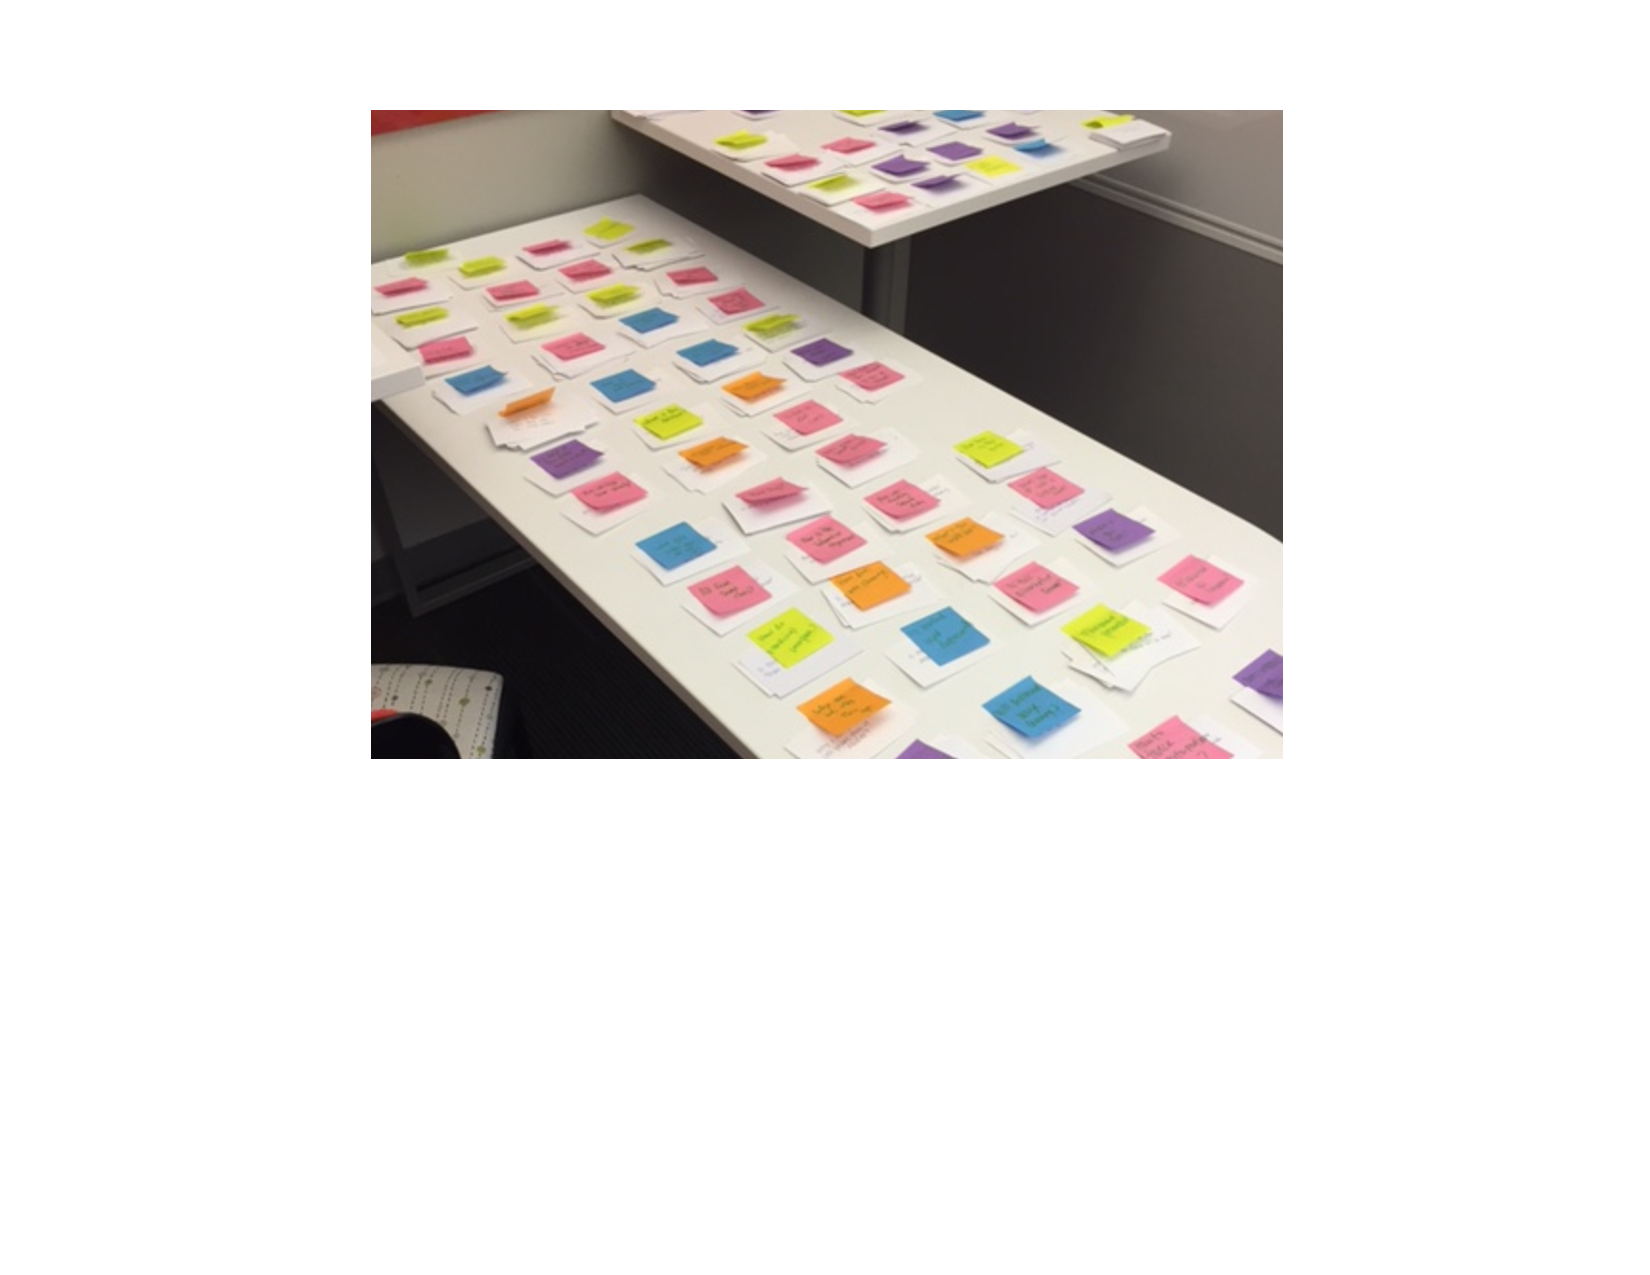
\includegraphics[width=3in]{Images/notecards.pdf}
\caption{Result of initial card sorting.}
\label{fig:cardsort} 
\end{figure}


We preformed our card sort in three stages. 
In the first stage we formed question clusters by grouping questions that identified the same information requirements (Figure~\ref{fig:cardsort}). 
For example, (EXAMPLES)

In the second stage we identified emergent themes and grouped the clusters into categories based on the themes. 
Table ?? contains the X categories along with the number of distinct clusters each contains.

To validate the categories we identified, DESCRIBE VERIFICATION STAGE! 

%https://www.interaction-design.org/encyclopedia/card_sorting.html

-Card Sorting
Dr. E Category validation?


\section{Results}
We extracted x questions, removing repeats, we came up with x questions


Question Category\\
-Example question\\
-Example question\\
-Example question\\

Description of questions in this category

\section{Discussion}
Data suggests that tools should focus on XYZ. Discuss categories and implications.

\section{Conclusion}
The conclusion goes here.




% conference papers do not normally have an appendix


% use section* for acknowledgement
\section*{Acknowledgment}


The authors would like to thank...


\bibliographystyle{IEEEtran}
% argument is your BibTeX string definitions and bibliography database(s)
\bibliography{iTrustInterviews}
%
% <OR> manually copy in the resultant .bbl file
% set second argument of \begin to the number of references
% (used to reserve space for the reference number labels box)




% that's all folks
\end{document}


